\chapter{Results, Conclusion and outlook}
In the last chapter we will present the final results and draw a conclusion of the work.
The chapter ends with an outlook on possible directions to continue and improve
the work done so far.

\section{Results}
Here we will present hopefully the interesting results achieved

For the final analysis a set of classroom profiles have been selected

\begin{itemize}
    \item \textbf{Class A:} Description
    \item \textbf{Class B:} ...
    \item \textbf{Class C:} ...
\end{itemize}

Comparing those classroom profile produces the following HA-Plot

\begin{figure}[H]
    \makebox[\textwidth][l]{%
    \begin{minipage}[t]{500pt}
        \centering
        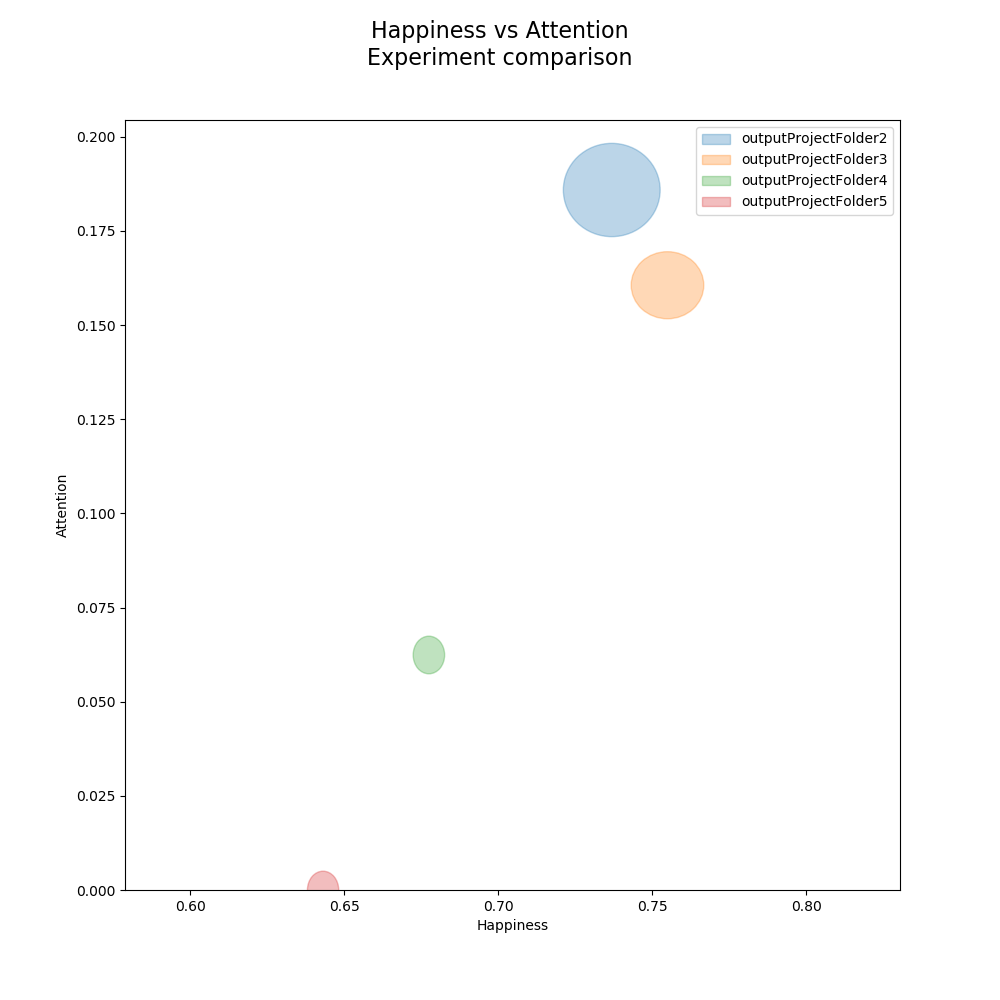
\includegraphics[width=400pt]{StudyResults}
        \caption{Final Study results}
        \label{StudyResults}
    \end{minipage}    
    }%
\end{figure}

This result can be interpreted to be ....

Bla bla bla

\dots


\section{Conclusion}
As part of this Thesis we where able to develop a multi-agent model that is simulation
a virtual classroom.

We have devised a Agent Logic that is based on the established Big-Five Personality
Trait model and that produces agent behavior consistent with empirical studies.

We have developed a data analysis pipeline that makes it possible to efficiently
run multiple simulations in a batch mode, enabling a statistical analysis of the
simulation results.

Based on the pedagogical literature about classroom dynamics we have selected a
set of interesting classroom profiles and compared their simulation results.

Doing so we found that \dots

The simulation software, the data analysis scripts and all content presented in this
work is available under the MIT License from the github repository \href{https://github.com/mapa17/breakfastclub}{https://github.com/mapa17/breakfastclub}.



\section{Outlook}
As mentioned shortly in the chapter on Objectives some initial objectives had to
be dropped during the development of the thesis in order to stay within the available
time frame.

The following is a list of possible improvements, as well as ideas for follow up projects.

\begin{itemize}
    \item \textbf{Interactive Simulation:} Making the simulation interactive, by being able to
    force agents to perform certain actions, expulse students from the classroom, call for silence
    or similar interactions would make it possible to develop a teacher training 
    program. Similar to commercial solutions like TLE TeachLive \cite{Dieker2017} or simSchool \cite{Badiee2015}
    but open source and with agent behavior that is based on a psychological model.
    
    \bb
    
    In order to support learning and provide a novel visualization of the effect
    of user interaction with the simulation we envisioned a system that is generating
    a clone of the running simulation when ever the user is performing an action.
    That clone would continue in a fast forward like matter to a defined simulation
    end can than be compared to the all other clones generated in the same way.
    This would make it possible to evaluate the effect of each user interaction
    onto the final result of the simulation.

    \item \textbf{Reinforcement trained teacher:} At the moment the simulation
    is consisting of only students that behave like an autonomous study group.
    With the teacher interactions described in the previous point about an interactive
    simulation, one could train a virtual teacher using reinforcement learning (RL) and
    the objective to maximize happiness and attention of the class.
    
    \bb

    As there is a fast amount of literature on different teaching methodologies,
    it would be interesting to study if the RL trained teacher applies any of the known
    methodologies or comes up with new ones. Another interesting aspect would be
    effect different classroom profiles have on the trained teacher. How different
    classroom profiles form and shape teacher behavior.

    \item \textbf{Screening of classroom profiles:} ...
    \item \textbf{Screening of classroom profiles:} ...
\end{itemize}